\documentclass{article}

\usepackage{graphicx}
\usepackage{tikz}
\usepackage{tikzsymbols}
\usetikzlibrary{calc,patterns,shapes.geometric}
\pagestyle{empty}
\usepackage[margin=0pt]{geometry}
\geometry{papersize={14in,12in}}

\def\centerarc[#1](#2)(#3:#4:#5){\draw[#1] ($(#2)+({#5*cos(#3)},{#5*sin(#3)})$) arc (#3:#4:#5);}

\begin{document}
	\begin{figure}
		\centering
		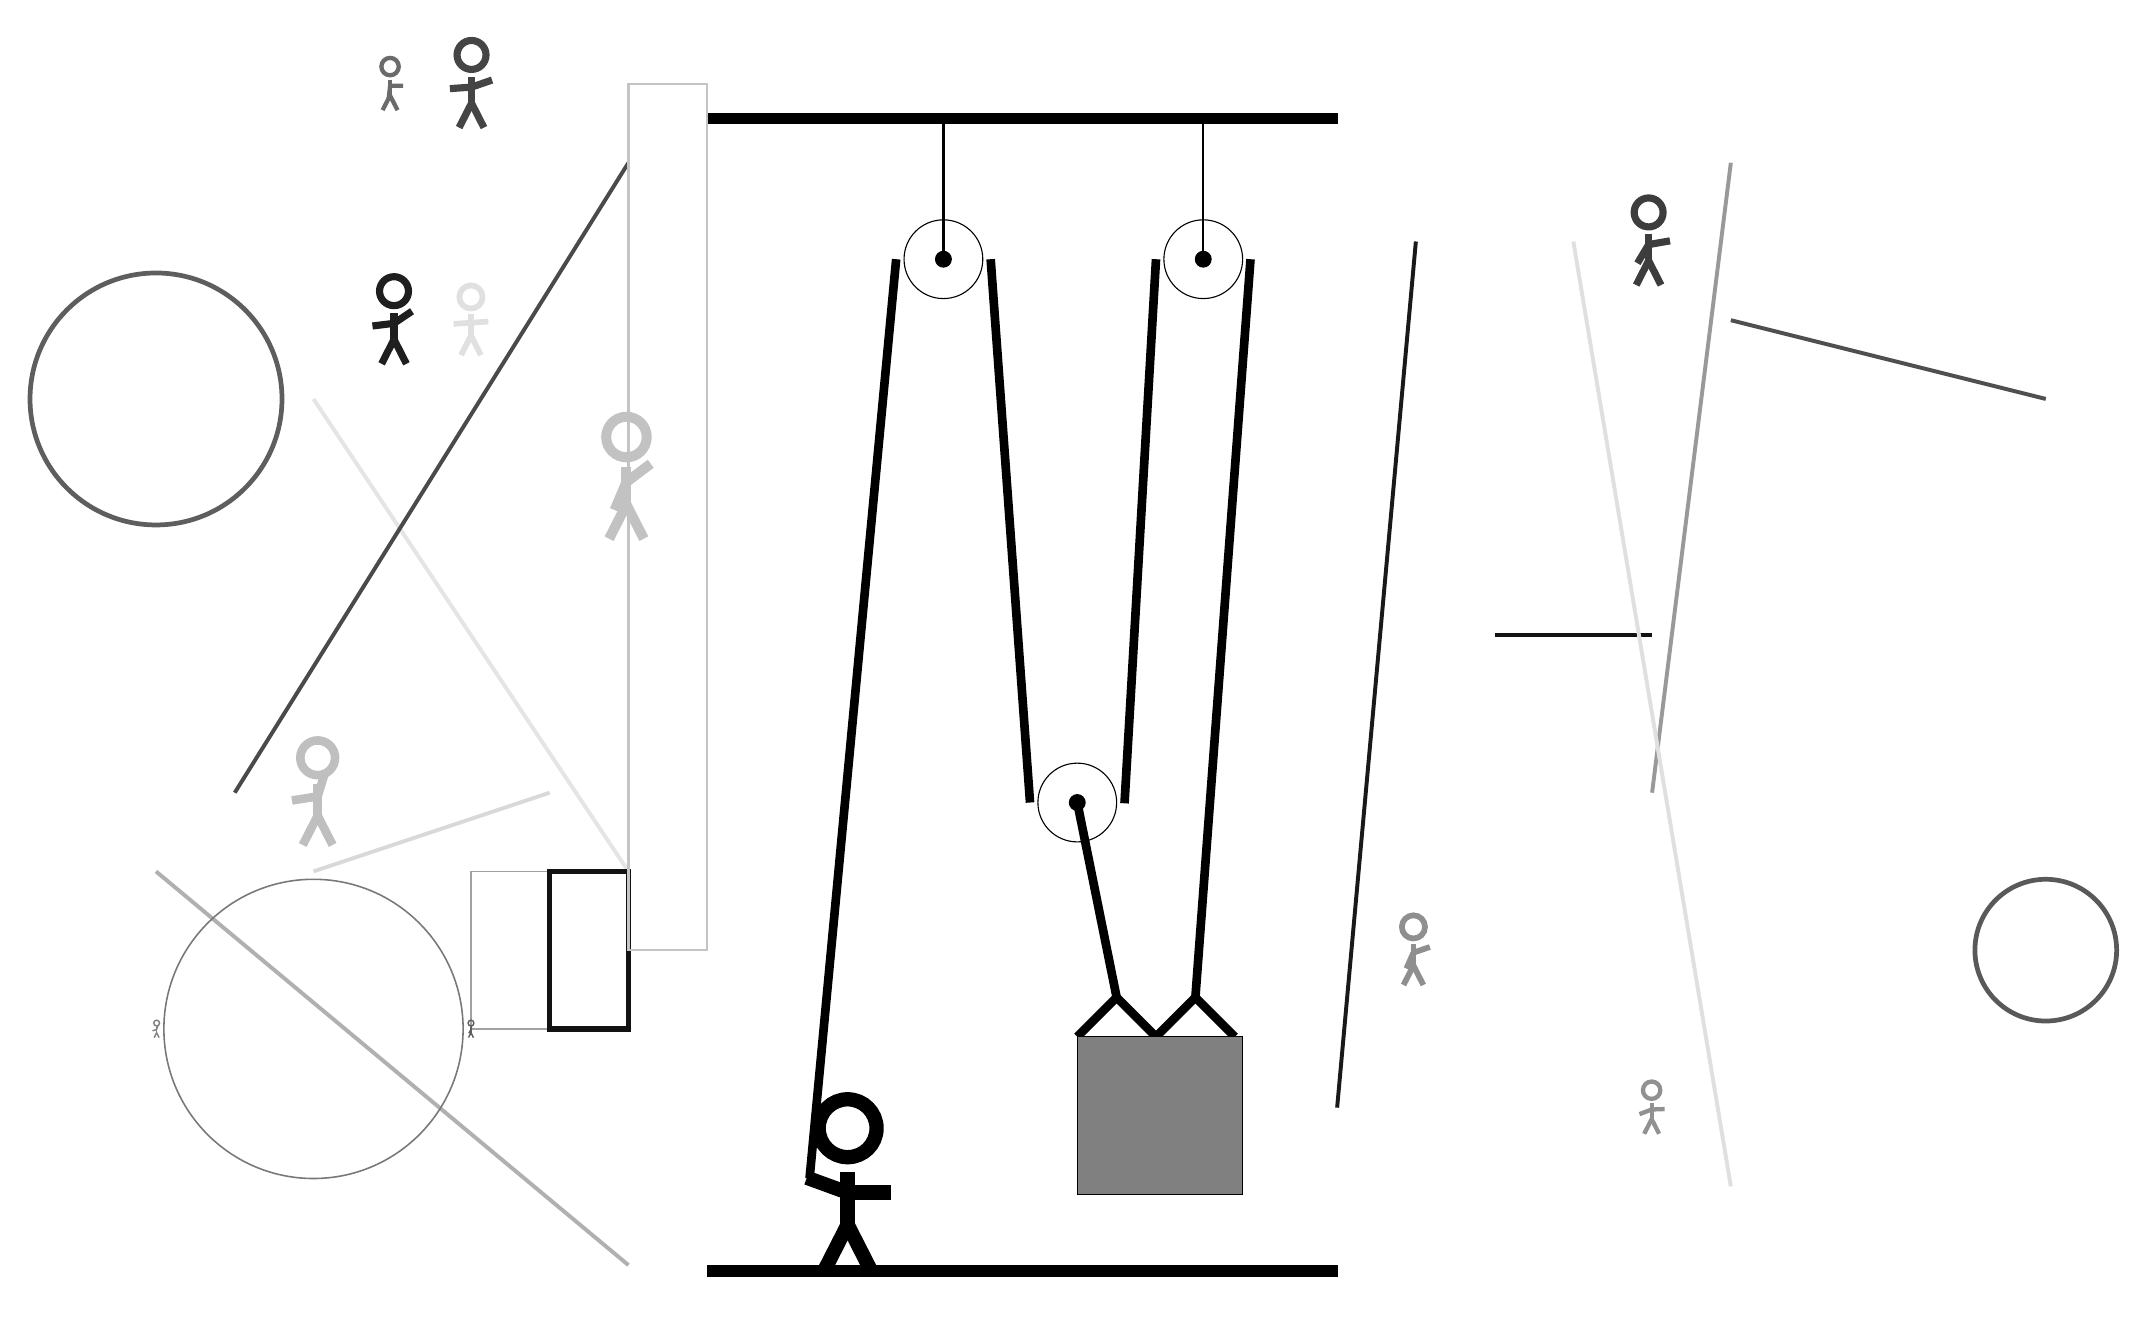
\begin{tikzpicture}
			%%%%% START %%%%%
			
			\draw[fill=black] (-2, 11.5) rectangle (6, 11.625);
			
			\draw (1, 9.775) circle (0.5);
			\draw[fill=black] (1, 9.775) circle (0.1);
			\draw[thick] (1, 9.775) -- (1, 11.5);
			
			\draw[line width=0.5mm, color=black!40](11, 11) -- (10, 3);
			
			\node[line width=0.5mm, color=black!58] at (-6, 12) {\Strichmaxerl[3][84][1]};
			\node[line width=0.4mm, color=black!44] at (7, 1) {\Strichmaxerl[4][66][19]};
			\node[line width=0.7mm, color=black!76] at (10, 10) {\Strichmaxerl[5][59][10]};
			\draw[line width=0.2mm, color=black!37] (-4, 0) rectangle (-5, 2);
			\draw[line width=0.5mm, color=black!10](-7, 8) -- (-3, 2);
			\draw[line width=0.5mm, color=black!31](-3, -3) -- (-9, 2);
			\node[line width=0.5mm, color=black!43] at (10, -1) {\Strichmaxerl[3][21][2]};
			\draw[line width=0.5mm, color=black!69](11, 9) -- (15, 8);
			\node[line width=0.2mm, color=black!25] at (-7, 3) {\Strichmaxerl[6][9][73]};
			
			\draw[line width=0.7mm, color=black!93] (-4, 0) rectangle (-3, 2);
			\draw[line width=0.5mm, color=black!90](7, 10) -- (6, -1);
			\draw[line width=0.5mm, color=black!15](-7, 2) -- (-4, 3);
			
			\draw[line width=0.5mm, color=black!71](-3, 11) -- (-8, 3);
			\draw[line width=0.3mm, color=black!23] (-3, 12) rectangle (-2, 1);
			\node[line width=0.5mm, color=black!50] at (-9, 0) {\Strichmaxerl[1][17][72]};
			\node[line width=0.3mm, color=black!73] at (-5, 12) {\Strichmaxerl[5][4][19]};
			\node[line width=0.7mm, color=black!24] at (-3, 7) {\Strichmaxerl[7][67][37]};
			\node[line width=0.4mm, color=black!63] at (-5, 0) {\Strichmaxerl[1][60][80]};
			
			\node[line width=0.5mm, color=black!88] at (-6, 9) {\Strichmaxerl[5][7][34]};
			\draw [line width=0.6mm, color=black!63](-9, 8) circle (1.6);
			
			\draw[line width=0.5mm, color=black!93](8, 5) -- (10, 5);
			
			\draw [line width=0.2mm, color=black!53](-7, 0) circle (1.9);
			\node[line width=0.6mm, color=black!12] at (-5, 9) {\Strichmaxerl[4][4][4]};
			\draw [line width=0.6mm, color=black!65](15, 1) circle (0.9);
			
			\draw[line width=0.5mm, color=black!12](9, 10) -- (11, -2);
			
			\draw (4.3, 9.775) circle (0.5);
			\draw[fill=black] (4.3, 9.775) circle (0.1);
			\draw[thick] (4.3, 9.775) -- (4.3, 11.5);
			
			\draw (2.7, 2.875) circle (0.5);
			\draw[fill=black] (2.7, 2.875) circle (0.1);
			
			\draw[line width=1.1mm]  (2.7, -0.1) -- (3.2, 0.4) -- (3.7, -0.1) -- (4.2, 0.4) -- (4.7, -0.1);
			\draw[fill=black!50] (2.7, -0.1) rectangle (4.8, -2.1);
			
			\draw[line width=1.1mm](-0.7, -1.9) -- (0.4, 9.775);
			\centerarc[line width=1.1mm](1, 9.775)(0:180:0.6);
			\draw[line width=1.1mm](1.6, 9.775) -- (2.1, 2.875);
			\centerarc[line width=1.1mm](2.7, 2.875)(180:370:0.6);
			\draw[line width=1.1mm] (3.3, 2.865) -- (3.7, 9.775);
			\centerarc[line width=1.1mm](4.3, 9.775)(0:180:0.6);
			\draw[line width=1.1mm](4.2, 0.4) -- (4.9, 9.775);
			\draw[line width=1.1mm] (3.2, 0.4) -- (2.7, 2.875);
			
			\node at (-0.2, -2) {\Strichmaxerl[10][-20][0]};
			
			\draw[fill=black] (-2, -3) rectangle (6, -3.15);
			
			%%%%% END %%%%%
		\end{tikzpicture}
	\end{figure}	
\end{document}